\documentclass[11pt,compress,t,notes=noshow, aspectratio=169, xcolor=table]{beamer}

\usepackage{../../style/lmu-lecture}
% Defines macros and environments
% This file is included in slides and exercises

% Rarely used fontstyle for R packages, used only in 
% - forests/slides-forests-benchmark.tex
% - exercises/single-exercises/methods_l_1.Rnw
% - slides/cart/attic/slides_extra_trees.Rnw
\newcommand{\pkg}[1]{{\fontseries{b}\selectfont #1}}

% Spacing helpers, used often (mostly in exercises for \dlz)
\newcommand{\lz}{\vspace{0.5cm}} % vertical space (used often in slides)
\newcommand{\dlz}{\vspace{1cm}}  % double vertical space (used often in exercises, never in slides)
\newcommand{\oneliner}[1] % Oneliner for important statements, used e.g. in iml, algods
{\begin{block}{}\begin{center}\begin{Large}#1\end{Large}\end{center}\end{block}}

% Don't know if this is used or needed, remove?
% textcolor that works in mathmode
% https://tex.stackexchange.com/a/261480
% Used e.g. in forests/slides-forests-bagging.tex
% [...] \textcolor{blue}{\tfrac{1}{M}\sum^M_{m} [...]
% \makeatletter
% \renewcommand*{\@textcolor}[3]{%
%   \protect\leavevmode
%   \begingroup
%     \color#1{#2}#3%
%   \endgroup
% }
% \makeatother


\title{Interpretable Machine Learning}
% \author{LMU}
%\institute{\href{https://compstat-lmu.github.io/lecture_iml/}{compstat-lmu.github.io/lecture\_iml}}
\date{}

\begin{document}

% Set style/preamble.Rnw as parent.

% Load all R packages and set up knitr

% This file loads R packages, configures knitr options and sets preamble.Rnw as 
% parent file
% IF YOU MODIFY THIS, PLZ ALSO MODIFY setup.Rmd ACCORDINGLY...

% Defines macros and environments
 \newcommand{\titlefigure}{figure/lime.png}
\newcommand{\learninggoals}{
\item Understand motivation for local explanations 
\item Develop an intuition for possible use-cases
\item Know characteristics of local explanation methods}

\lecturechapter{Introduction to local Explanations}
\lecture{Interpretable Machine Learning}

% ------------------------------------------------------------------------------

\begin{vbframe}{Methodological Motivation}
Except for Shapley values and ICE curves, we focused so far mostly on global explanation methods that explain global model behavior (e.g. PDP, PFI, etc.). However, there are also many methods that explain the \textbf{local} behavior of a model.
	\begin{itemize}
		\item Some local methods provide insight into the driving factors for a \textbf{particular decision}.
		\item Others help to understand the model's decision making in a \textbf{local environment} of the input space.
		\item Local Methods can address questions such as: 
		\begin{itemize}
		    \item \textbf{Why} did the model decide $\yh$ for input $\xv$?
		    \item \textbf{How} decides the model for cases similar to $\xv$?
		    \item \textbf{What} would the ML model have decided if $\xv$ differed in $\Xspace$?
		    \item  \textbf{Where} does the model fail?
		\end{itemize}  
	\end{itemize}
\end{vbframe}

\begin{vbframe}{Social Motivation}
All these questions can indeed be relevant for the ML modeler. However, unlike in global methods that require expert ML understanding or even domain knowledge, many local methods aim to provide explanations also for laypersons. 
	\begin{itemize}
		\item Explanations for laypersons must be tailored for the \textbf{explainee} (the person receiving the explanation).
		\item Thus, such explanations should be case specific, easy for humans to understand, and faithful to the explained mechanism.
		\item In particular if algorithms make decisions in \textbf{socially/safety critical domains}, end users have justified interest in receiving explanations.
		\item Local Explanations can not only increase \textbf{user trust}, but also help to detect \textbf{critical local biases} in algorithmic decision making.
		\item European citizens have the legally binding \textbf{right to explanation} as given in the General Data Protection Regulation (GDPR).

	\end{itemize}
\end{vbframe}


\begin{vbframe}{GDPR: The Right to Explanation}
    ``The data subject should have the right not to be subject to a decision, which may include a measure, evaluating personal aspects relating to him or her which is based solely on automated processing and which produces legal effects concerning him or her or similarly significantly affects him or her, such as automatic refusal of an online credit application or e-recruiting practices without any human intervention.

$\cdots$

In any case, such processing should be subject to suitable safeguards, which should include specific information to the data subject and the \textbf{right} to obtain human intervention, to express his or her point of view, \textbf{to obtain an explanation of the decision reached after such assessment and to challenge the decision}.
'' \\[0.2cm] (\href{https://gdpr-text.com/read/recital-71/}{Recital 71, GDPR})
\end{vbframe}


\begin{vbframe}[allowframebreaks]{Example: Husky or Wolf?}
	\begin{itemize}
		\item We trained a model to predict if an image shows a wolf or a husky. 
		\item Below the predictions on six test images are given. 
		\item Do you trust our predictor? 
	\end{itemize}
	\begin{center}
		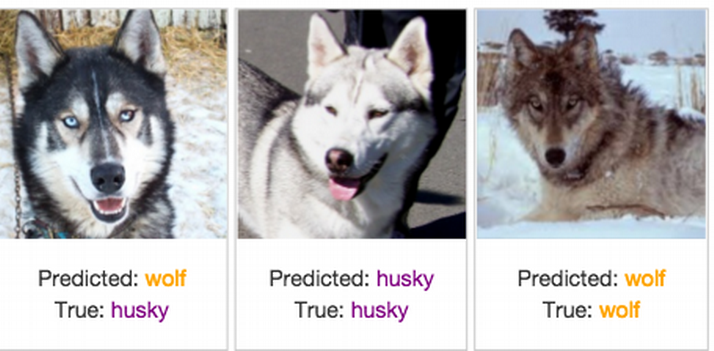
\includegraphics[width=0.35\textwidth]{figure/lime-wolfhusky.png}\\
		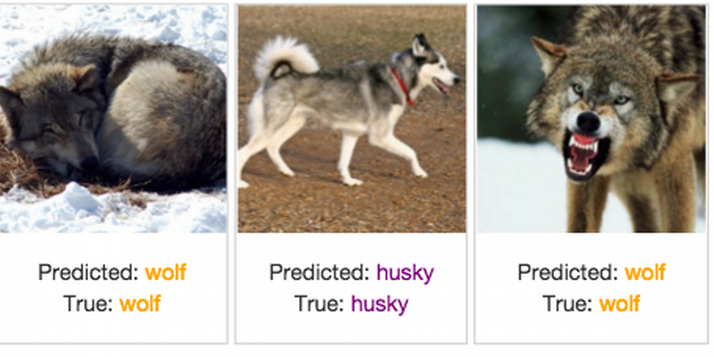
\includegraphics[width=0.35\textwidth]{figure/lime-wolfhusky2.png}\\
		%{\tiny \textbf{Source:} \href{http://www.facweb.iitkgp.ac.in/~niloy/COURSE/Spring2018/IntelligentSystem/PPT_2018/why_should_i_trust_ppt.pdf}{Sameer Singh (2018)}}
	\end{center}
	
	\begin{itemize}
		\item We can use local explanations (in this case LIME) to highlight the parts of an image which led to the prediction.
		\item We can see that our predictor is actually a snow detector. 
	\end{itemize}
	\begin{center}
		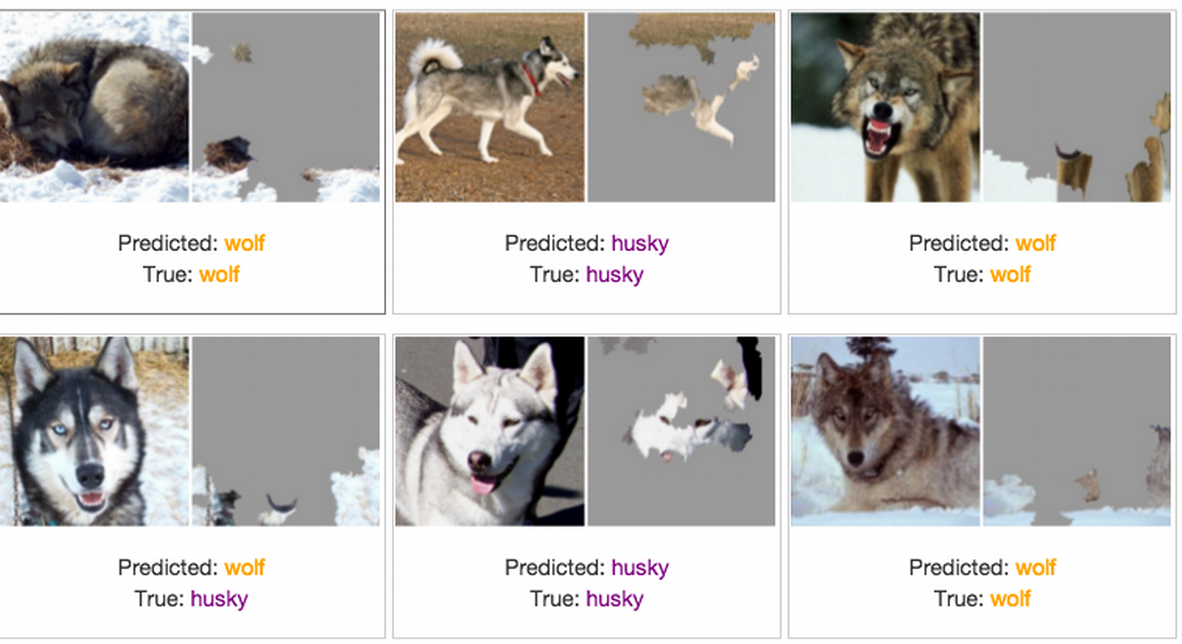
\includegraphics[width=0.75\textwidth]{figure/lime-wolfhusky3.png}\\
		{\tiny \textbf{Source:} \href{http://www.facweb.iitkgp.ac.in/~niloy/COURSE/Spring2018/IntelligentSystem/PPT_2018/why_should_i_trust_ppt.pdf}{Sameer Singh (2018)}}
	\end{center}
\footnote[frame]{Sameer Singh (2018). Explaining Black-Box Machine Learning Predictions.  \url{http://www.facweb.iitkgp.ac.in/~niloy/COURSE/Spring2018/IntelligentSystem/PPT_2018/why_should_i_trust_ppt.pdf}.}
\end{vbframe}

\begin{vbframe}{Example: Loan Application}
Assume you are applying at a bank's online portal for a loan and your application gets immediately rejected without reasons.
	\begin{center}
		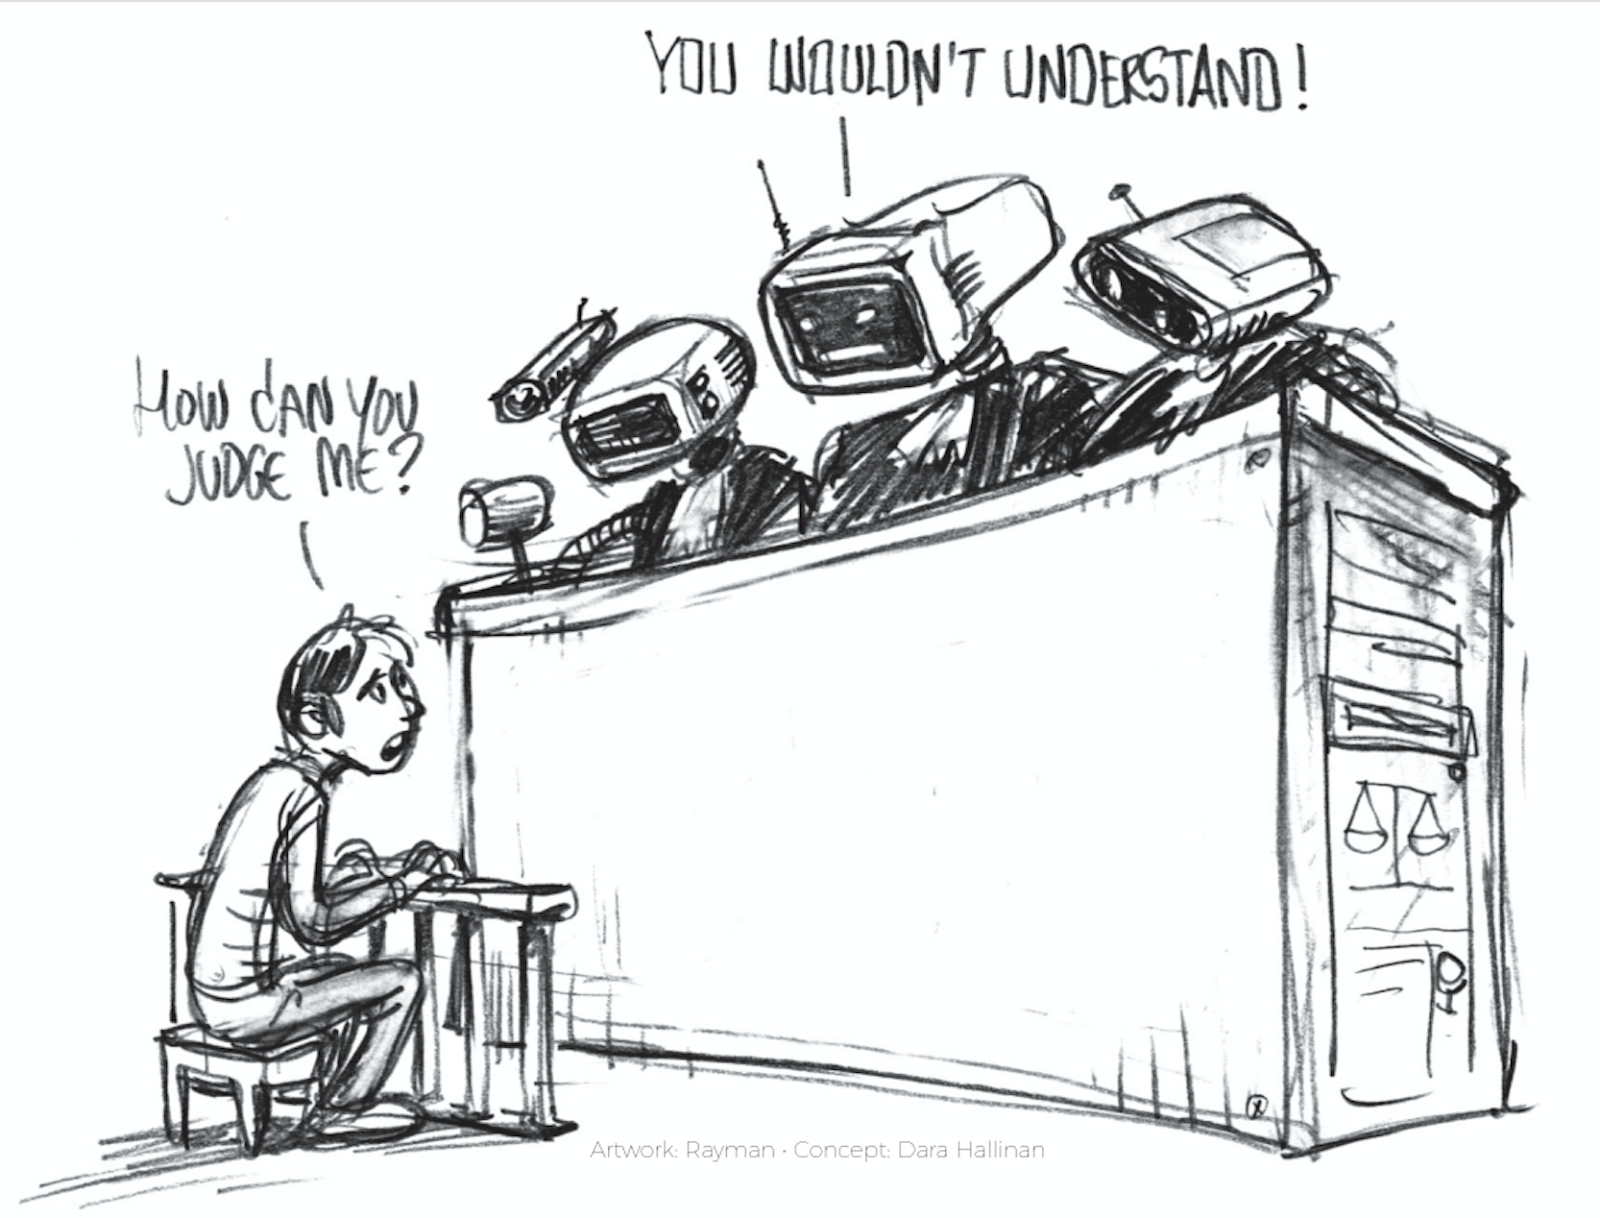
\includegraphics[width=0.4\textwidth]{figure/IntroJudge.png}\\
		{\tiny \textbf{Source:} \href{https://www.elte.hu/content/trendfordulo-az-mi-fejlesztesekben.t.19025}{https://www.elte.hu}}
	\end{center}
	If the bank would use local explanation methods, it could e.g. provide a counterfactual explanation:
	\begin{itemize}
	    \item[] ``If you were older than 21, your loan application would have been accepted."
	\end{itemize}
\end{vbframe}

\begin{vbframe}{Example: Stop or Right-of-Way?}
Assume you work in a car company and are about to use an image classifier for autonomous driving. Then, you show your model the following image (an adversarial example). The classifier is $99\%$ sure it describes a right-of-way sign.
	\begin{center}
		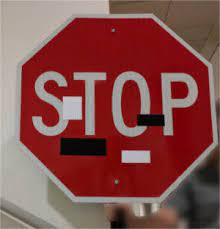
\includegraphics[width=0.3\textwidth]{figure/IntroStop.jpg}\\
		{\tiny \textbf{Source:} Eykholt et. al (2018)}
	\end{center}
	Would you entrust other peoples lives into the hands of this software?
	\footnote[frame]{Eykholt, Kevin et al. (2018). Robust Physical-World Attacks on Deep Learning Visual Classification. \\1625-1634. 10.1109/CVPR.2018.00175.}
\end{vbframe}

\begin{vbframe}{Characteristics}
	\begin{itemize}
		\item \textbf{Explanation scope:} Specific prediction, local environment.
		\item \textbf{Model classes:} Mostly model-agnostic in definition but model-specific for computational reasons, very popular also for deep learning models.
		\item \textbf{Audience:} ML modelers and laypersons.
		\item \textbf{Data types:} Many, including tabular, image, text and audio data.
		\item \textbf{Methods:} Many, most prominent are counterfactual explanations, shapley values, local interpretable model-agnostic explanations (LIME), adversarial examples, single ICE curve, anchors.
		\item \textbf{Special:} Due to audience, strong interactions with social sciences. Also, strong connections to cognitive science and neurosciences due to data types.
	\end{itemize}
\end{vbframe}

\begin{vbframe}{Recap: ICE Curve}
		\begin{itemize}
		\item ICE curves visualize how the model prediction $\fh(\xv)$ of a individual observation $\xv$ change by varying the feature values of one or two features while keeping all other features fixed. 
		\item ICE curves must be interpreted with care for highly correlated features or feature regions with a few observations. 
	\end{itemize}
\vspace{0.5cm}
\begin{columns}
	\begin{column}{0.47\textwidth}
		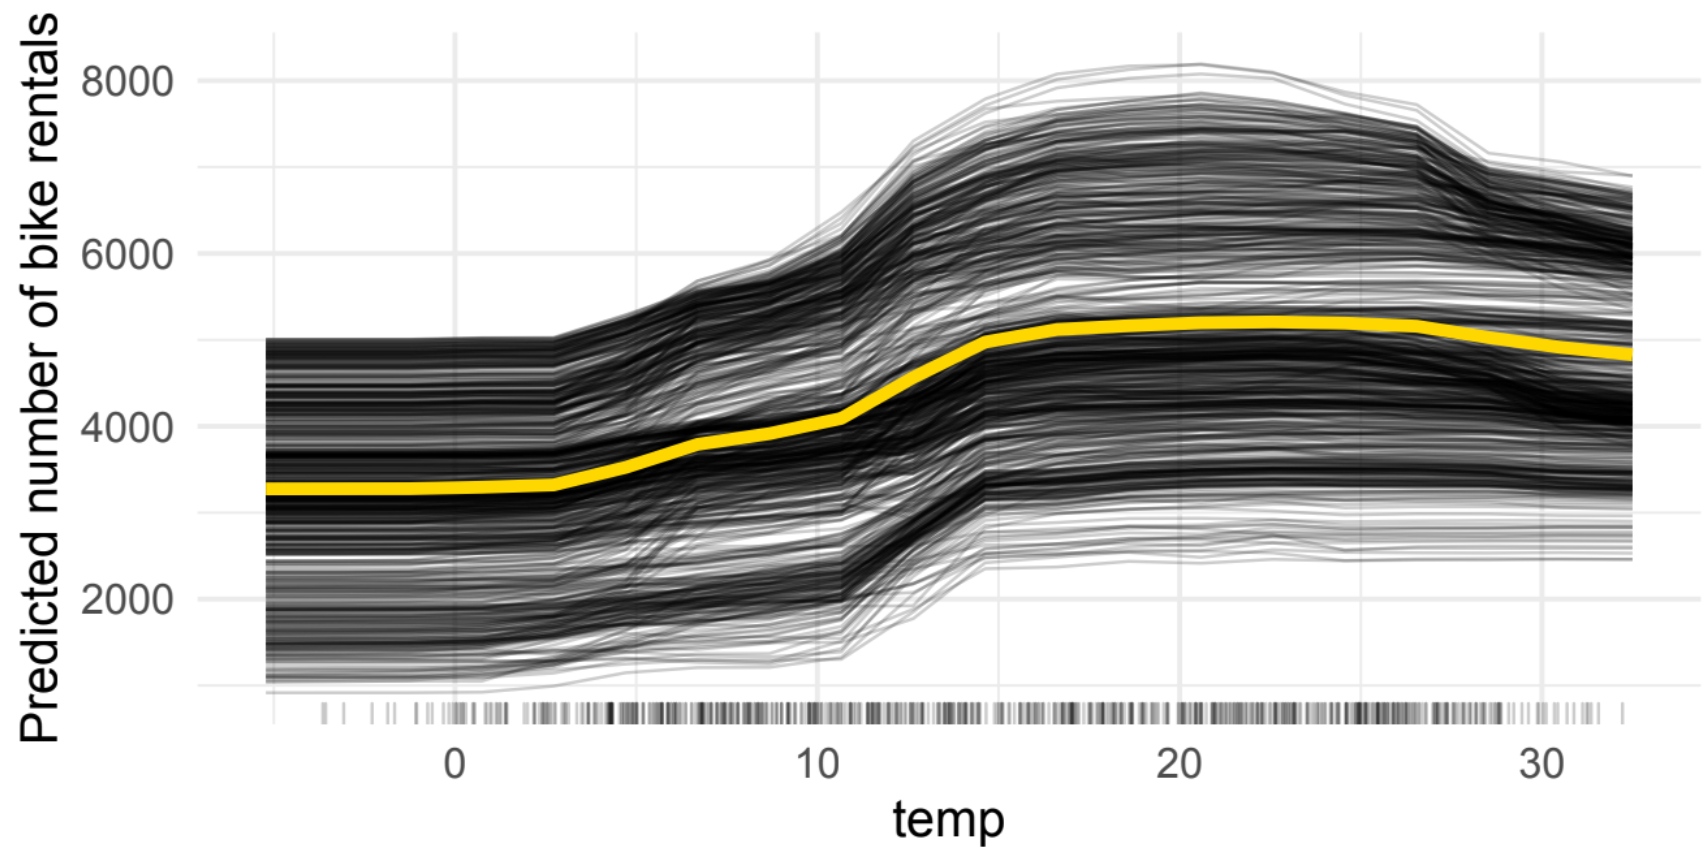
\includegraphics[width=1\textwidth]{figure/bike-sharing-dataset01.png}
	\end{column}
	\begin{column}{0.47\textwidth}
		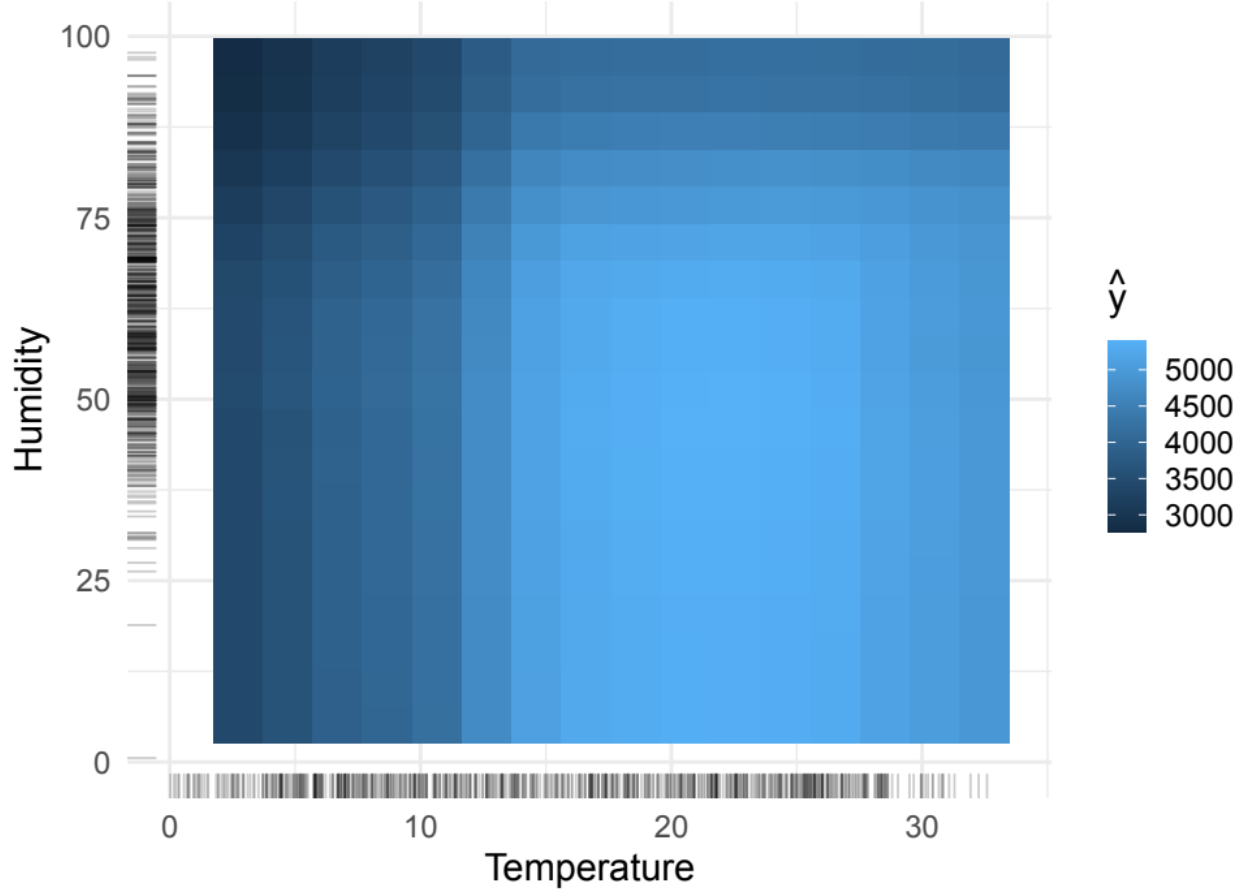
\includegraphics[width=1\textwidth]{figure/bike-sharing-dataset02.png}
	\end{column}
\end{columns}
\end{vbframe}

\begin{vbframe}{Recap: Shapley Values}
	\begin{itemize}
		\item Shapley values were original proposed in game theory.
		\item They are a local explanation method because they tell us how each feature $x_j$ contributes to the overall prediction $\fh(\xv)$ of a specific observation $\xv$. 
	\end{itemize}
\vspace{0.5cm}
\begin{center}
	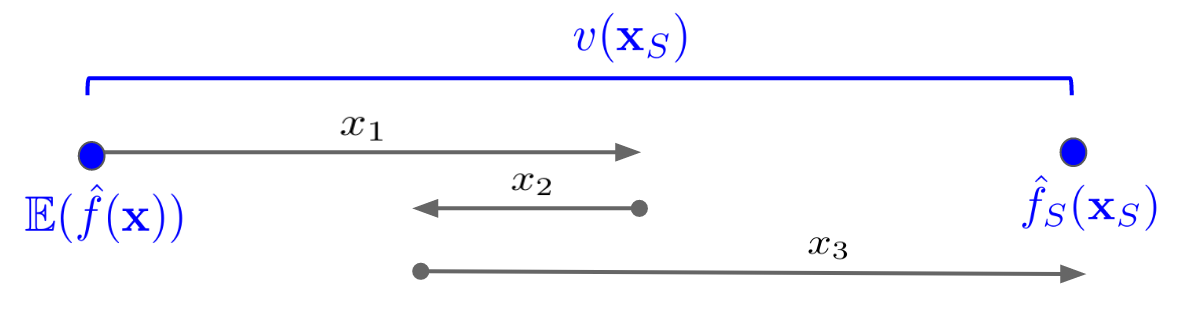
\includegraphics[width=0.8\textwidth]{figure/shapley_valuefct}
\end{center}
\end{vbframe}

\begin{vbframe}{Credit Dataset}

	\begin{itemize}
		\item In this section, we demonstrate local explanation methods on the German credit classification dataset from Kaggle. \href{https://www.kaggle.com/uciml/german-credit}{\beamergotobutton{Click here}}
		\item The dataset has 522 complete observations and nine features containing credit and customer information.
		\item The binary target indicates whether a customer has a `good' or `bad' credit risk.  
		\item We combined categories with few case numbers. 
	\end{itemize}
		\begin{center}
			\footnotesize
			\begin{tabular}{ccc}
				\hline
				name & type & range\\
				\hline
				age & numeric & [19, 75]\\
				sex & factor & \{male, female\}\\
				job & factor & \{0, 1, 2, 3\}\\
				housing & factor & \{free, own, rent\}\\
				saving.accounts & factor & \{little, moderate, rich\}\\
				checking.accounts & factor & \{little, moderate, rich\}\\
				credit.amount & numeric & [276, 18424]\\
				duration & numeric &  [6, 72]\\
				purpose & numeric &  \{others, car, furniture, radio/TV\}\\
				risk & factor & \{good, bad\}
			\end{tabular}
		\end{center}
\end{vbframe}

\endlecture
\end{document}
